%!TEX root = paper.tex
\subsection{Structural estimates}
The estimation results are given in \Cref{table: estimates (min_size=3 max_size=5 margin=2000)}.
\begin{table}[H]
\centering
\caption{Estimates of Parameters ($3 \leq |\mathbf{C}_i| \leq 5$)}
\label{table: estimates (min_size=3 max_size=5 margin=2000)}
\begin{tabular}{cccc}
\toprule
Calibrated $\alpha$ & Parameters & Estimates & Standard Error \\
\midrule
0.33 & $\beta$ & 0.449 & 0.033 \\
 & $\sigma$ & 172.305 & 26.501 \\
0.5 & $\beta$ & 0.459 & 0.034 \\
 & $\sigma$ & 176.316 & 25.023 \\
0.67 & $\beta$ & 0.494 & 0.039 \\
 & $\sigma$ & 180.203 & 25.898 \\
\bottomrule
\end{tabular}
\end{table}


The estimates of governments'
revenue share $\beta$ and the scale parameter of the error term $\sigma$ are stable.
$\hat{\beta}$ varies from 0.45 to 0.51, $\hat{\sigma}$ varies from 172 to 182
for all three different capital income shares.
\hyperref[sec:robustness checks 1]{Appendix B.1}
presents the estimation results under the two settings of $3 \leq |\mathbf{C}_i| \leq 4$ and
$4 \leq |\mathbf{C}_i| \leq 5$, and $\hat{\beta}$ varies from 0.53 to 0.58 for the first case,
$\hat{\beta} \approx 0.4$ for the second case. Thus, even if each firm has
4 or 5 candidate cities, i.e., the fiscal competition is very fierce,
the estimates of $\beta$ don't vary far from $\estbeta$. And $\hat{\beta} = \estbeta$
is a conservative estimate for the governments' revenue share since if I decrease the sizes of
the choice sets, $\hat{\beta}$ will be higher than 0.5.
\hyperref[sec:robustness checks 2]{Appendix B.2} presents the estimation results under the
different settings of action spaces of city governments,
and it also shows $\hat{\beta} = \estbeta$ is a conservative estimate.

To conclude, $\alpha=0.5$ is a valid calibrated value,
and $\hat{\beta} = \estbeta, ~\hat{\sigma} = \estsigma$ are my preferred estimates.
I will use these estimates in the remaining analysis of the paper.



\subsection{Discussion of the estimation results}
\label{subsec:discussion of results}
As \Cref{table: estimates (min_size=3 max_size=5 margin=2000)} shows,
the city governments' revenue share of firms' output is quite high
($\hat{\beta} \approx \estbeta$),
which is consistent with my assumption that attracting industrial firms
to land in a city's jurisdiction will generate huge potential benefits for the city government
by the fiscal externality or spill-over effects.

To clearly illustrate this point, a thought experiment can be considered:
I assume the only benefits city governments can get from landing new firms
is the value-added tax (VAT) revenue and
the city government officials think they can get the benefits in five years
after the new firm landed.\footnote{
    Five years is an overestimated term since the average term for
    Chinese city communist party secretary and mayor are 3.6 years and 3.2 years respectively
    during 2000-2010, see \url{https://www.yicai.com/news/3106338.html}.}

I also assume the labor income is 70\% of firms' output,
which might be an overestimation since $\alpha = 0.3$ in this case.
Since the average profit ratio of industrial firms in 2012 is 6\%,\footnote{
    This profit ratio (6\%) is calculated by the National Bureau of Statistics of China, see
    \url{http://www.stats.gov.cn/tjsj/zxfb/201301/t20130127_12932.html}.}
I can assume the taxable added value is 80\% (greater than 70\% $+$ 6\%) of the firms' output,
which is also an overestimated figure.

The VAT rate is 17\%,
the share of city government in VAT revenue is 25\%, and the back-of-envelop
calculation shows that the city government's revenue share is
$5 \times 80\% \times 17\% \times 25\% = 0.17$, which is 38\% of
$\hat{\beta} \approx \estbeta$.\footnote{
    According to a survey conducted by Chinese Academy of Fiscal Sciences,
    the ratio of firm tax to added value is around 6.6\% in 2013,
    see \url{http://www.cf40.com/news_detail/7374.html}, which is much lower than
    $80\% \times 17\% = 13.6\%$, thus, my comparison is very conservative.
}
Thus, attracting new firms brings city governments a huge amount of
benefits such as promoting local business,
boosting the housing market, etc. besides the official tax revenue. The fiscal externality of attracting industrial firms is huge.


\subsection{Fit of the model}
To check whether my model describes the fiscal competition between city governments
properly,
I discuss the fit of the model in this section.

I compare the distributions of observed land prices and simulated land prices
in \Cref{fig: cdf_fit} and \Cref{table: fit_of_model}.

\begin{figure}[H]
    \centering
    \caption{Comparison of empirical CDFs of observed land prices and simulated land prices}
    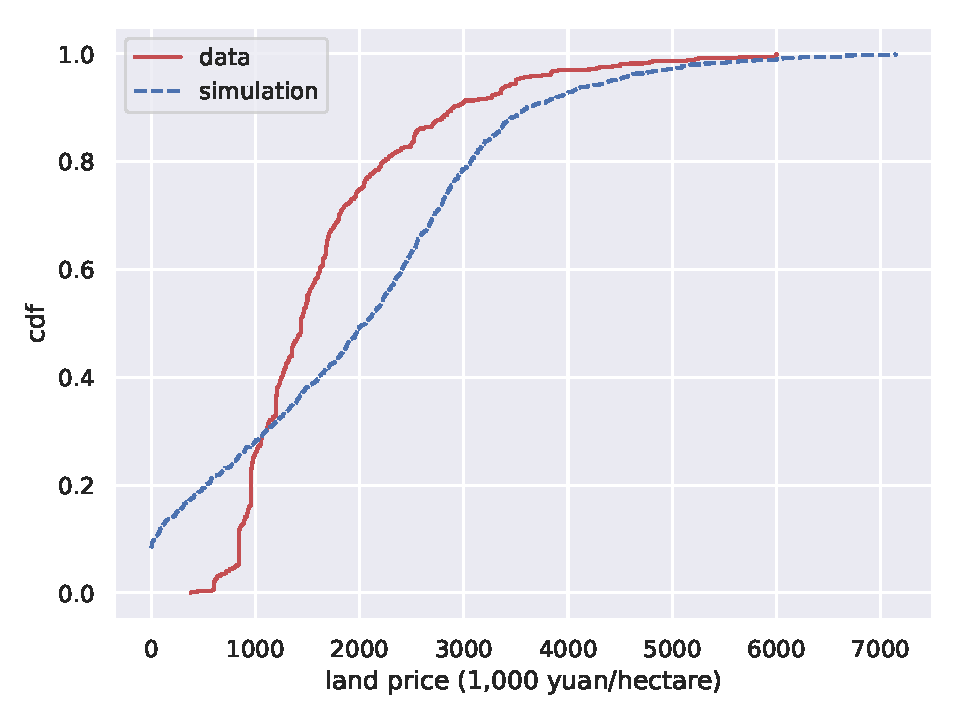
\includegraphics[scale=0.7]{\graphs/cdf_data_sim.pdf}
    \fnote{Notes: I use the preferred estimates to do 30 simulations,
        and use the average of the expected land price in these simulations
        as the simulated land price.}
    \label{fig: cdf_fit}
\end{figure}
\Cref{fig: cdf_fit} shows the empirical CDFs of both observed land prices and simulated land prices.
And the two empirical CDFs are close though there are more high prices in simulation.

\begin{table}[H]
\centering
\caption{Descriptive Statistics of Observed Prices and Simulated Prices}
\label{table: fit_of_model}
\begin{tabular}{lcc}
\toprule
 & observed price & simulated price \\
\midrule
mean & 1685.097 & 1986.903 \\
std & 934.952 & 1397.491 \\
min & 379.505 & 0.000 \\
25% & 978.617 & 833.703 \\
50% & 1440.007 & 2049.601 \\
75% & 2015.520 & 2864.467 \\
max & 6001.559 & 7144.140 \\
\bottomrule
\end{tabular}
\end{table}

\Cref{table: fit_of_model} shows the descriptive statistics of the observed prices
and simulated prices.
The mean and 25\% percentile of simulated prices are matched well to observed prices.
But the standard deviation, median, and 75\% percentile of simulated prices are not matched well to
observed prices. This is because my model is parsimonious, and
may not explain the second-order moment of land price very well.
Another reason for the relatively poor matches of the median and 75\% percentile of land prices
is that I don't use the higher-order moments
in the estimation, since higher-order moments are difficult to be precisely computed within
a finite number of observations \citep{adda2003dynamic}. However, since the matches of the
mean and 25\% percentile are good, I proceed to use the preferred estimates
for the counterfactual analysis.


